%----------------------------------------------------------
% PACKAGES AND THEMES
%----------------------------------------------------------
\documentclass[aspectratio=169,xcolor=dvipsnames,handout]{beamer}

\usetheme{Darmstadt}
\usecolortheme{seahorse}
\setbeamercovered{transparent}
\setbeamertemplate{footline}[frame number]

\usepackage[hangul]{kotex}
\usepackage{hyperref,graphicx, array, adjustbox, makecell}

% other packages
\usepackage{natbib}
\usepackage{float,pstricks,listings,stackengine,xcolor,calligra}
\usepackage{amsmath,amssymb,latexsym}
\usepackage{booktabs,longtable,multicol,multirow,lscape,rotating}
\usepackage{caption,subcaption}
%\newcommand{\source}[1]{\subcaption*{\raggedright 자료: {#1} } }
\usepackage{threeparttable} % Align column caption, table, and notes
\usepackage{adjustbox} % Shrink stuff
%\usepackage{showframe} % Useful for debugging

% defs
\def\cmd#1{\texttt{\color{red}\footnotesize $\backslash$#1}}
\def\env#1{\texttt{\color{blue}\footnotesize #1}}
\definecolor{deepblue}{rgb}{0,0,0.5}
\definecolor{deepred}{rgb}{0.6,0,0}
\definecolor{deepgreen}{rgb}{0,0.5,0}
\definecolor{halfgray}{gray}{0.55}

\lstset{%
    basicstyle=\ttfamily\small,
    keywordstyle=\bfseries\color{deepblue},
    emphstyle=\ttfamily\color{deepred},    % Custom highlighting style
    stringstyle=\color{deepgreen},
    numbers=left,
    numberstyle=\small\color{halfgray},
    rulesepcolor=\color{red!20!green!20!blue!20},
    frame=shadowbox,
}

\hypersetup{unicode=true,colorlinks=true,linkcolor=blue}

% font조정
%\usepackage{fontspec}
%\setmainfont{Times New Roman}
%\setmainhangulfont{NanumGothic}

% 문자열 대체{노사관계론 전용}
\usepackage{newunicodechar}
\newunicodechar{•}{\textperiodcentered}
\newunicodechar{➔}{$\implies$}
\newunicodechar{∴}{$\therefore$}
\newunicodechar{∵}{$\because$}

%----------------------------------------------------------
% TITLE PAGE
%----------------------------------------------------------
\title{한국의 다차원적 불평등 현황 분석 및 관련 지수 개발}
\subtitle{한국의 교육불평등 분석}
\author{오성재(한국보건사회연구원)}
\institute[KIHASA]
    {%
        국회입법조사처
    }
\date{2025년 9월 16일}

%----------------------------------------------------------
\begin{document}
%----------------------------------------------------------

\frame{\titlepage}

\begin{frame}{목차}
    \setcounter{tocdepth}{1}
    \tableofcontents
\end{frame}

\section{들어가는 말}
\begin{frame}[<+->]
\frametitle{측정의 대상}
    \begin{itemize}
        \item 교육의 불평등은 측정의 대상에서 특수성을 지님.
        \begin{itemize}[<+->]
            \item 경제력(소득, 부)는 개인의 성취가 매 시점에 바뀌는데, 교육성취는 생에 특정시점에 고정됨.
            \item 경제력(소득, 부)는 측정단위가 화폐로 동일한데, 교육성취는 단위가 상이함.
            \item 교육년수, 시험점수 또는 우수기관 진학여부 등.
        \end{itemize}
    \end{itemize}
\end{frame}

\begin{frame}[<+->]
\frametitle{교육자료}
    \begin{itemize}
        \item 완벽한 교육분야 자료는 존재.
        \begin{itemize}[<+->]
            \item 소득의 경우 국세청을 포함한 그 어떤 기관이나 주체도 정확한 파악이 어려움.
            \item 반면, 교육분야에서는 행정기관이 대부분의 정보를 파악하고 있음.
                \begin{itemize}[<+->]
                    \item 학적부, 생기부, NICE, 수능점수 등등.
                \end{itemize}
            \item 최종적으로 이러한 교육분야 행정데이터를 접근가능하게 해야.
        \end{itemize}
        \item 각종 종단자료 존재.
        \begin{itemize}[<+->]
            \item 국가단위 종단연구.
            \item 시도단위 : 서울교육종단연구, 부산교육종단연구 등등.
            \item 매년마다 학년이 바뀌기 때문에 종단자료도 완벽하지 않음.
        \end{itemize}
        \item 국제 교육자료.
        \begin{itemize}[<+->]
            \item TIMSS, PISA, PIAAC 등등.
        \end{itemize}
    \end{itemize}
\end{frame}

\begin{frame}[<+->]
\frametitle{연구내용}
    \begin{itemize}
        \item 역대 정부에서 지속된 교육서비스의 양적 확대에 대하여 소개.
        \begin{itemize}[<+->]
            \item 현재 한국은 개인의 의사에 의한 진학에 충분한 교급별 교육서비스를 공급.
        \end{itemize}
        \item 한국은 최빈국에서 선진국으로 이행하면서 교육불평등의 대상이 바뀜.
        \begin{itemize}[<+->]
            \item 과거는 교육년수 위주.
            \item 교육에서의 성취는 단순한 고등교육 진학이 아닌, 우수대학·우수학과로의 진학으로 바뀜.
        \end{itemize}
    \end{itemize}
\end{frame}

\section{교육자원의 공급확대}
\begin{frame}[<+->]
    \begin{figure}
        \centering
        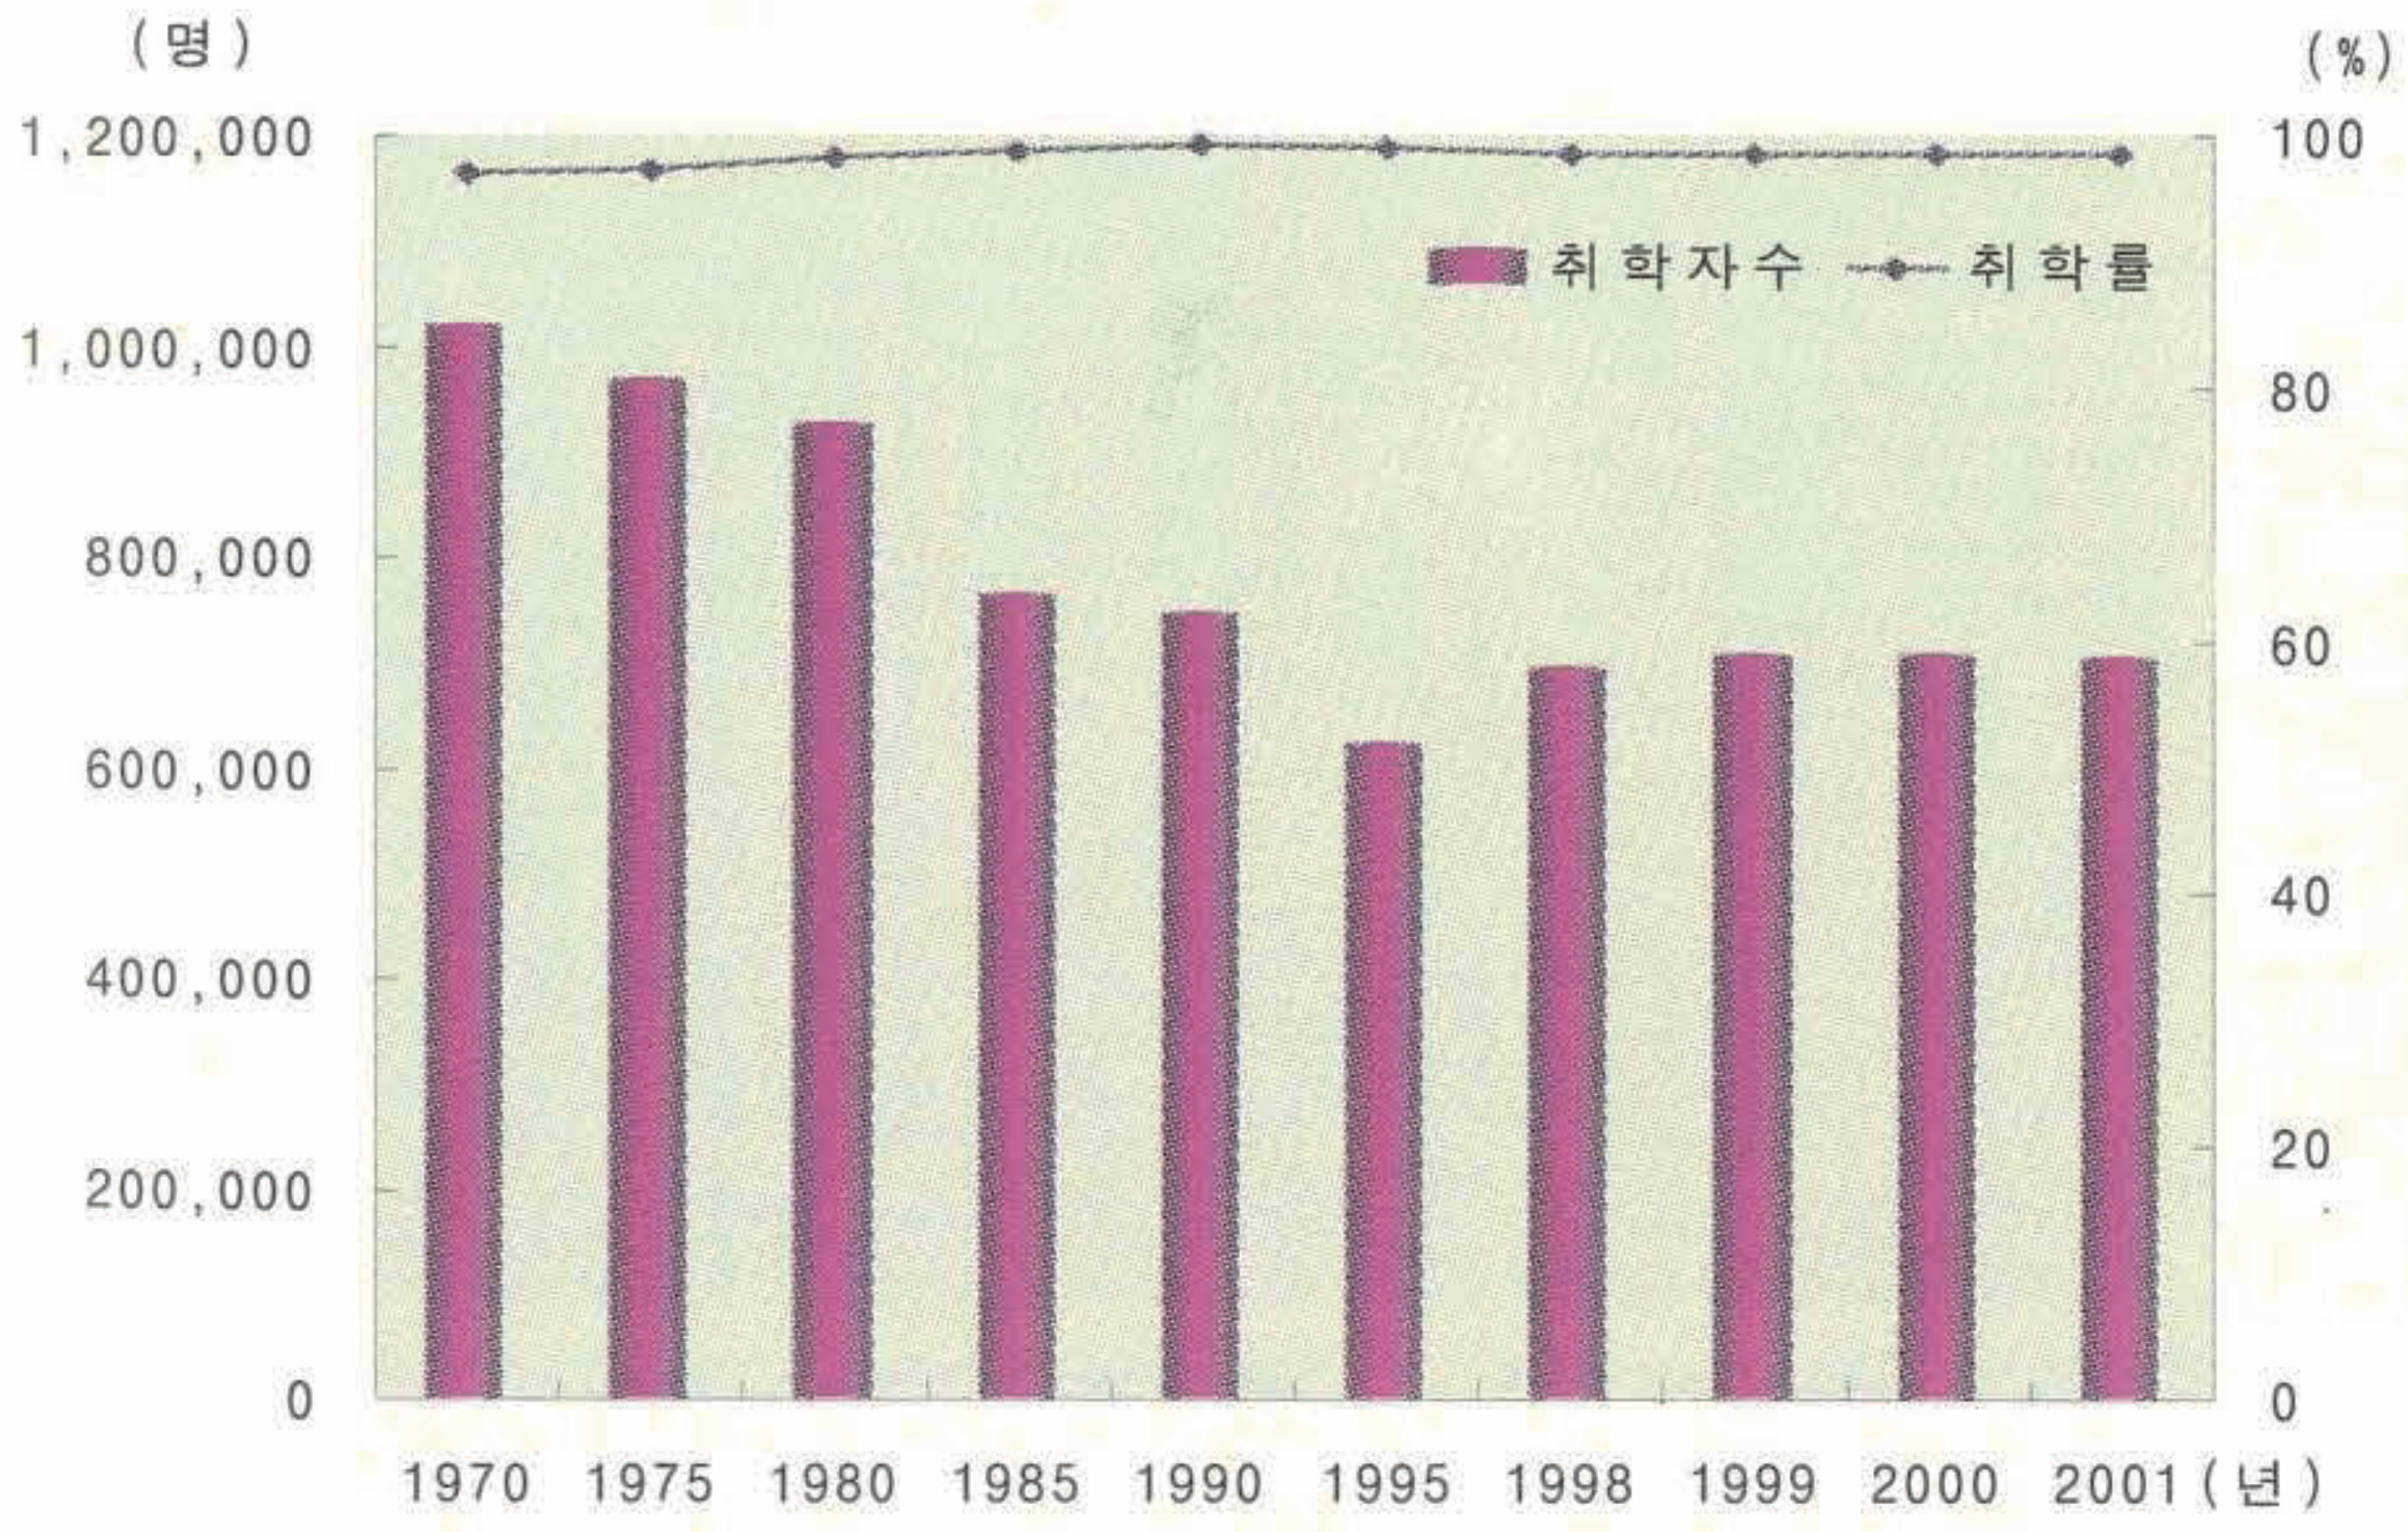
\includegraphics[width=.4\textwidth]{pic/edus1.png}
        \\
        \raggedright%
        \hspace{1.5em}
        \tiny{자료: 한국교육개발원 (1998), 간추린 교육통계.}
        \caption{초등학교 취학률, 1965--1998}
    \end{figure}
    \begin{itemize}
        \item 초등학교 취학률은 70년에도 90\% 이상임.
    \end{itemize}
\end{frame}

\begin{frame}[<+->]
    \begin{figure}
        \centering
        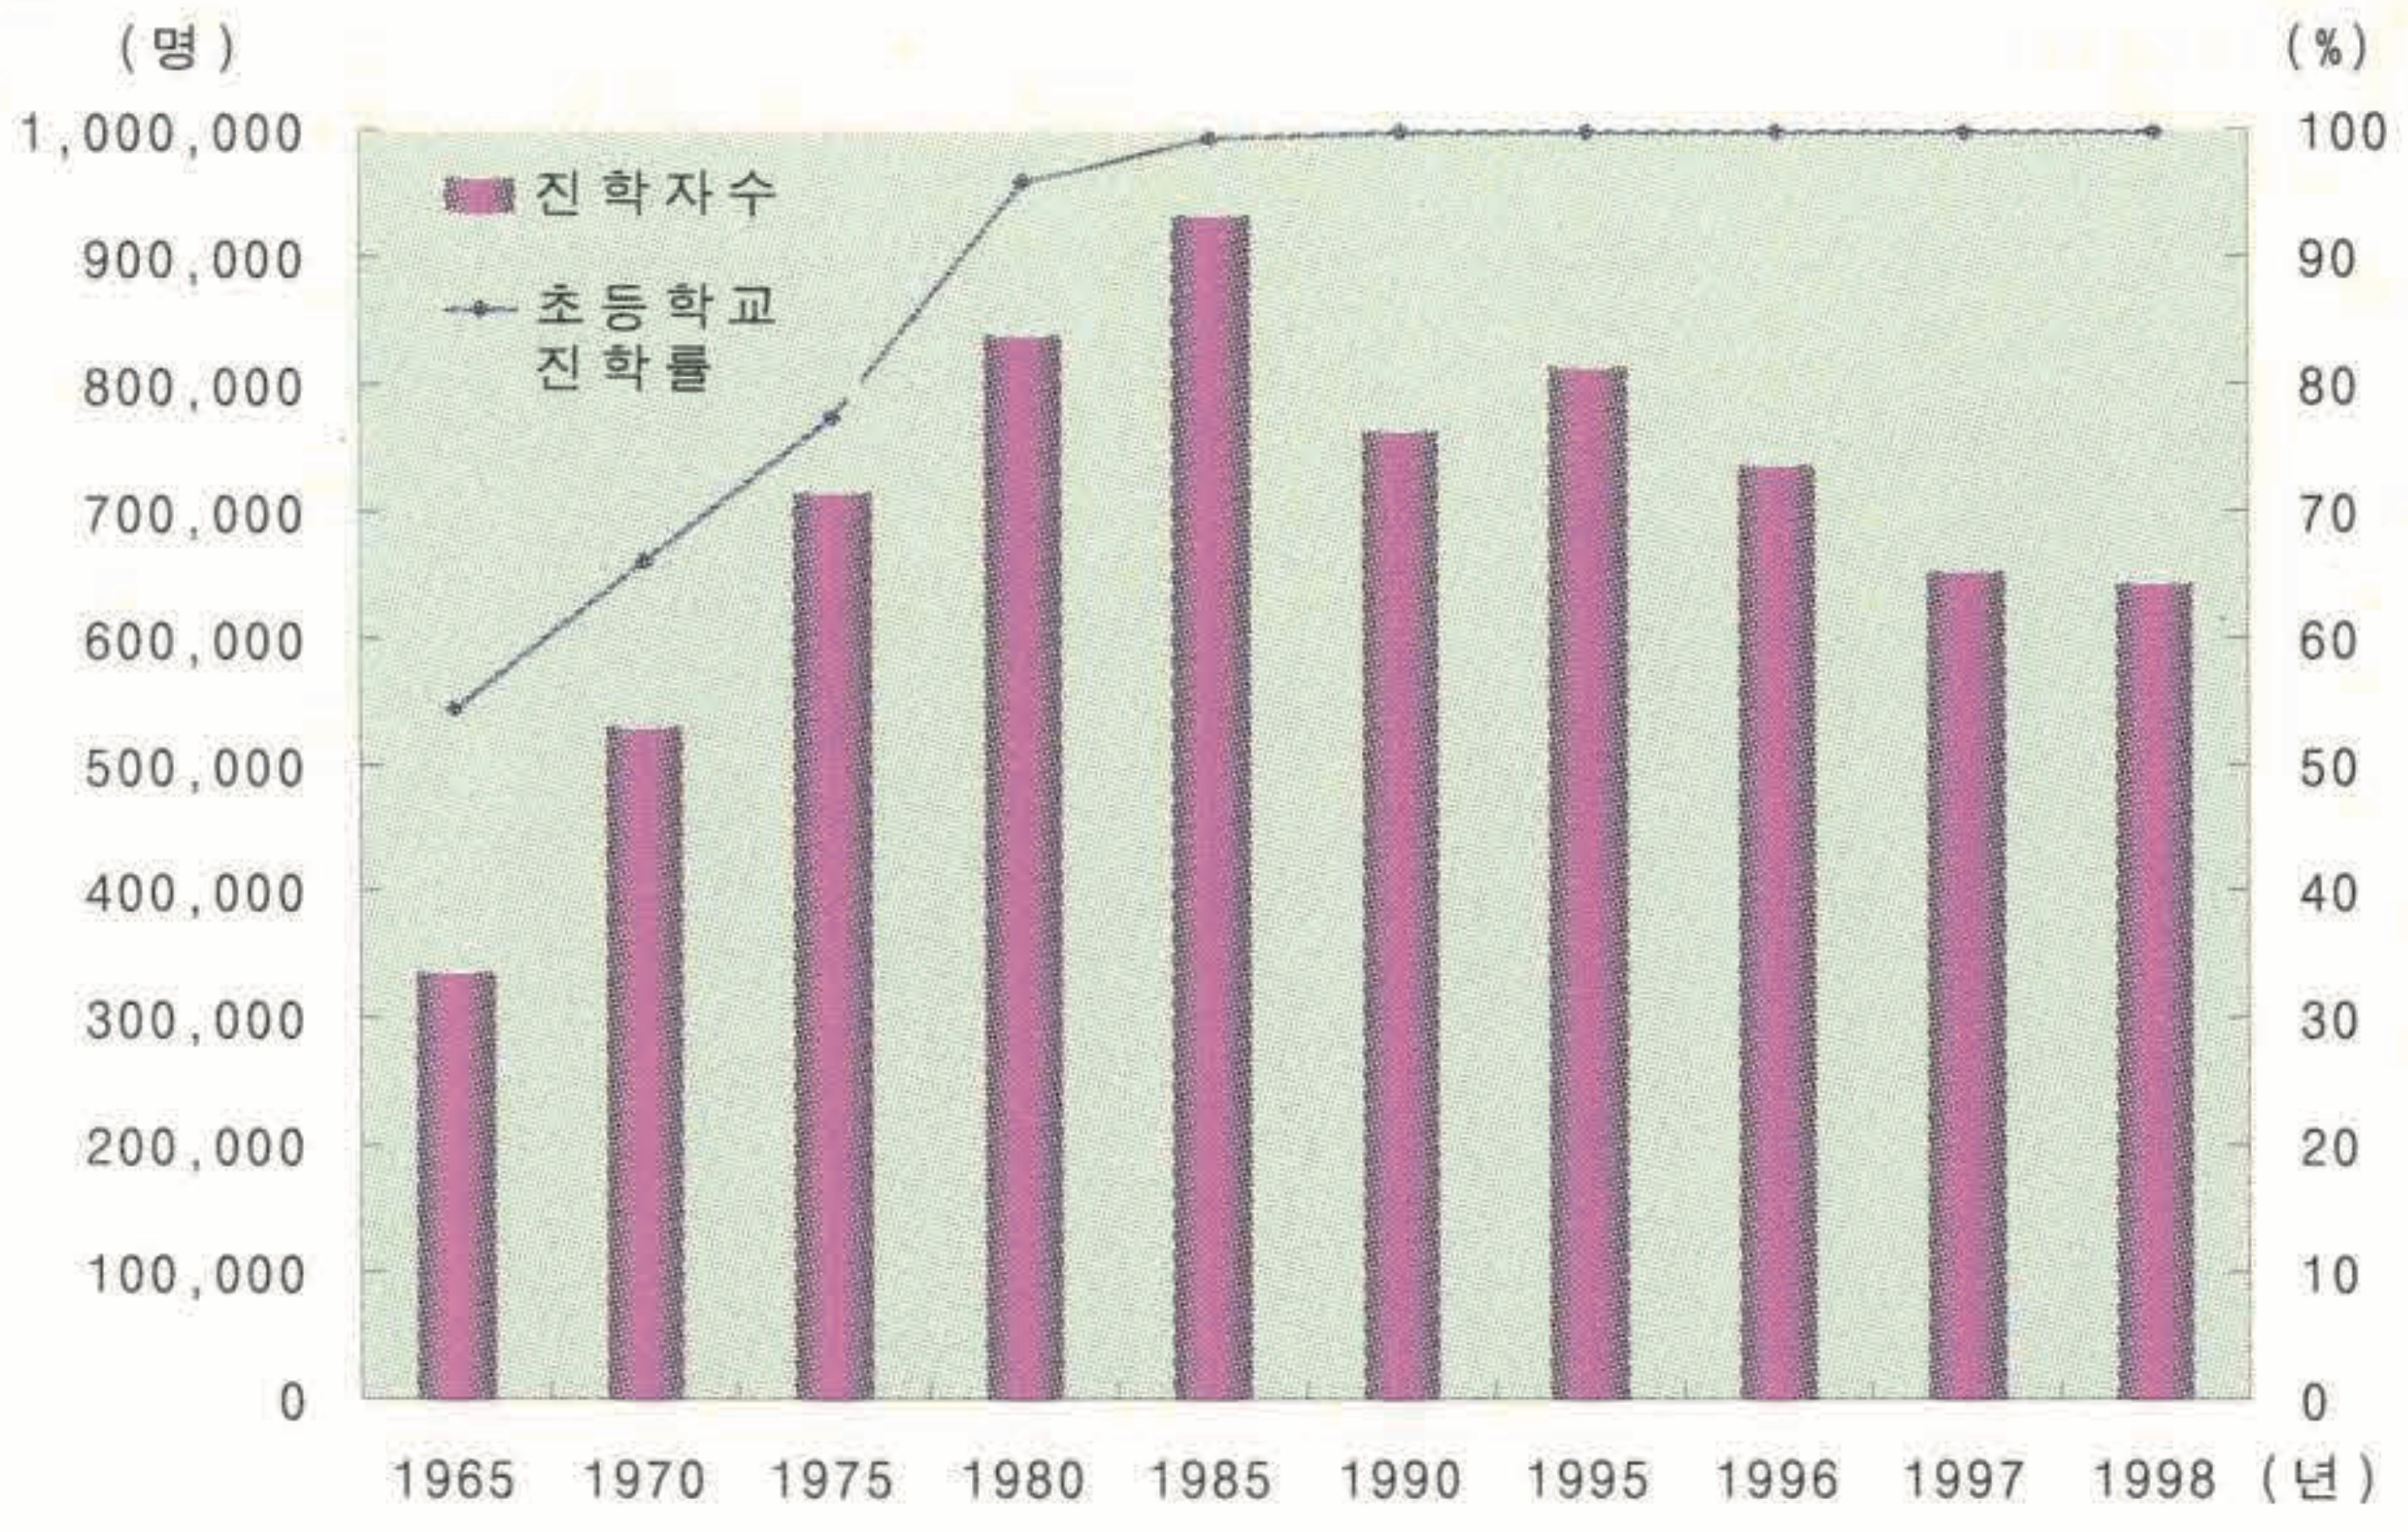
\includegraphics[width=.4\textwidth]{pic/edus2.png}
        \\
        \raggedright%
        \hspace{1.5em}
        \tiny{자료: 한국교육개발원 (1998), 간추린 교육통계.}
        \caption{초등학교 졸업자 진학률, 1965--1998}
    \end{figure}
    \begin{itemize}
        \item 초등학교 졸업자의 진학률은 85년이 되어야 100\%에 근접.
    \end{itemize}
\end{frame}

\begin{frame}[<+->]
    \begin{figure}
        \centering
        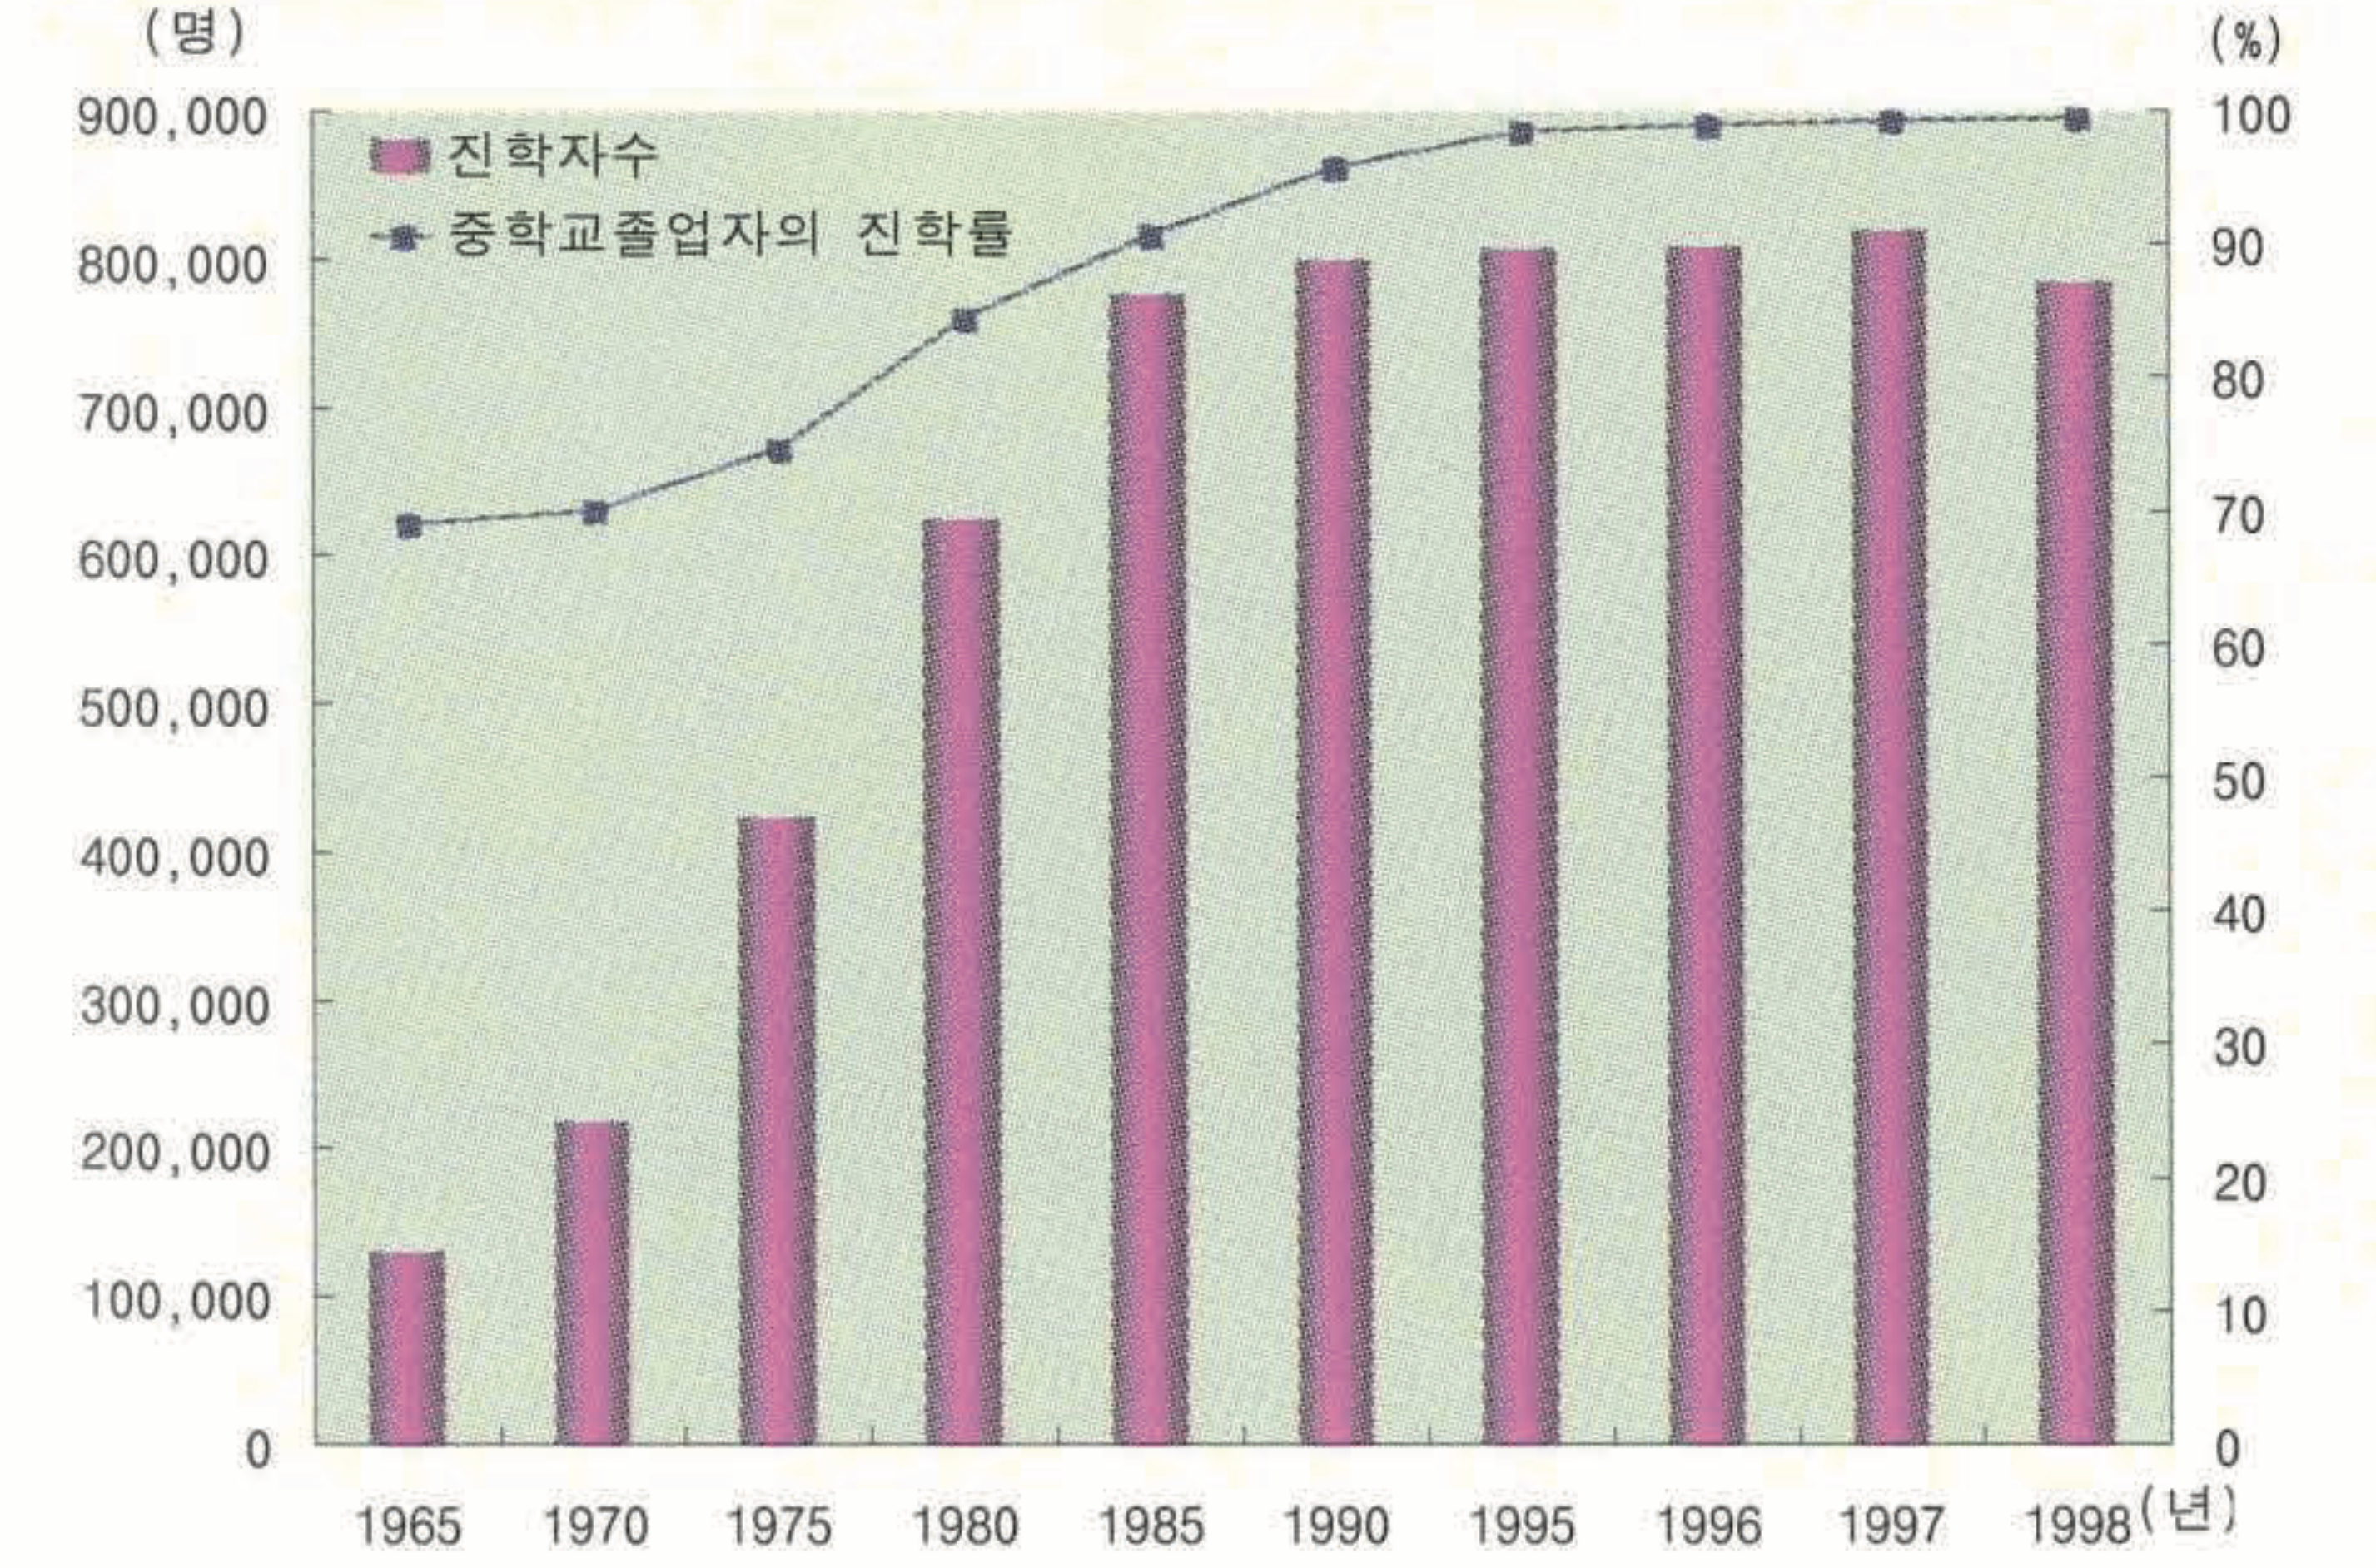
\includegraphics[width=.4\textwidth]{pic/edus3.png}
        \\
        \raggedright%
        \hspace{1.5em}
        \tiny{자료: 한국교육개발원 (1998), 간추린 교육통계.}
        \caption{중학교 졸업자 진학률, 1965--1998}
    \end{figure}
    \begin{itemize}
        \item 중학교 졸업자의 진학률은 95년 98.5\%.
    \end{itemize}
\end{frame}

\begin{frame}[<+->]
    \begin{table}
        \centering
        \resizebox{.7\textwidth}{!}{\relax
            \begin{tabular}{|c|c|c|c|c|c|c|c|c|c|c|c|}
\hline
\multicolumn{2}{|c|}{구분} & 1965 & 1970 & 1975 & 1980 & 1985 & 1990 & 1995 & 1996 & 1997 & 1998 \\ \hline
\multirow{3}{*}{학급당 학생수} 
 & 초등학교 & 65.4 & 62.1 & 56.7 & 51.5 & 44.7 & 41.4 & 36.4 & 35.7 & 35.1 & 34.9 \\ \cline{2-12}
 & 중학교   & 60.7 & 62.1 & 64.5 & 62.1 & 61.7 & 50.2 & 48.2 & 46.5 & 43.6 & 40.8 \\ \cline{2-12}
 & 고등학교 & 57.1 & 58.2 & 58.6 & 59.8 & 56.9 & 52.8 & 47.9 & 48.7 & 49.3 & 48.2 \\ \hline
\multirow{3}{*}{교원 1인당 학생수} 
 & 초등학교 & 62.4 & 56.9 & 51.8 & 47.5 & 38.3 & 35.6 & 28.2 & 27.6 & 27.3 & 27.4 \\ \cline{2-12}
 & 중학교   & 39.4 & 42.3 & 43.2 & 45.1 & 40.0 & 25.4 & 24.8 & 23.8 & 22.3 & 20.9 \\ \cline{2-12}
 & 고등학교 & 30.2 & 29.7 & 31.4 & 33.3 & 31.0 & 24.6 & 21.8 & 22.1 & 22.4 & 22.0 \\ \hline
\multirow{2}{*}{초등학교 2부제 학급수} 
 & 대도시(광역시이상) & - & 2,050 & 902 & 5,188 & 2,804 & 4,579 & 914 & 731 & 437 & 381 \\ \cline{2-12}
 & 기타지역 & - & 5,507 & 385 & 5,547 & 2,651 & 3,356 & 712 & 664 & 536 & 460 \\ \hline
\multirow{3}{*}{진학률 (\%)} 
 & 초등학교→중학교 & 54.3 & 66.1 & 77.2 & 95.8 & 99.2 & 99.8 & 99.9 & 99.9 & 99.9 & 99.9 \\ \cline{2-12}
 & 중학교→고교     & 69.1 & 70.1 & 74.7 & 84.5 & 90.7 & 95.7 & 98.5 & 99.0 & 99.4 & 99.5 \\ \cline{2-12}
 & 고교→고등교육기관 & 32.3 & 26.9 & 25.8 & 27.2 & 36.4 & 33.2 & 51.4 & 54.9 & 60.1 & 64.1 \\ \hline
\multirow{4}{*}{취업률 (\%)} 
 & 일반계고 & 31.6 & 17.3 & 16.9 & 15.7 & 16.2 & 18.7 & 26.4 & 24.8 & 22.0 & 18.5 \\ \cline{2-12}
 & 실업계고 & 43.4 & 56.4 & 56.1 & 58.2 & 60.4 & 84.0 & 90.9 & 91.8 & 91.7 & 84.7 \\ \cline{2-12}
 & 전문대학 & 57.5 & 72.6 & 58.3 & 50.3 & 57.2 & 71.8 & 74.2 & 78.2 & 75.5 & 66.3 \\ \cline{2-12}
 & 대학교   & 44.0 & 70.6 & 71.8 & 73.0 & 52.1 & 55.0 & 60.9 & 63.3 & 61.8 & 50.5 \\ \hline
\end{tabular}

        }
        \\
        \raggedright%
        \hspace{1.5em}
        \tiny{자료: 한국교육개발원 (1998), 간추린 교육통계.}
        \caption{연도별 교육지표, 1965--1998}
    \end{table}
\end{frame}

\begin{frame}[<+->]
    \begin{figure}
        \centering
        \includegraphics[width=.4\textwidth]{pic/edus4.png}
        \\
        \raggedright%
        \hspace{1.5em}
        \tiny{자료: 한국교육개발원 (2024), 간추린 교육통계.}
        \caption{연도별 교육단계별 진학률, 2000--2024}
    \end{figure}
    \begin{itemize}
        \item 고교졸업자의 대학진학은 05년 73.4\% 이후로 안정됨.
    \end{itemize}
\end{frame}

\section{교육의 양적 불평등}
\begin{frame}[<+->]
\frametitle{양적불평등 분석}
    \begin{itemize}[<+->]
        \item 교육은 공평하게 받더라도 그 결과는 개인마다 상이함.
        \begin{itemize}[<+->]
            \item 타고난 능력, 가족의 지원, 그밖의 환경요인 등등.
            \item 전국 1등, 시험 100점, 명문대 수석입학 등등.
        \end{itemize}
        \item 교육단계별 완전 진학에 도달하는 시점이 상이.
        \item 초기에는 교육의 불평등을 양적으로 측정해야. 
        \item 교육적 성취는 본인에게 내재되지만, 그 자원은 부모로 부터.
        \item 따라서 부모의 속성이 자녀의 교육적 성취에 영향을 주지 않아야.
    \end{itemize}
\end{frame}

\begin{frame}[<+->]
\frametitle{한국노동패널}
    \begin{itemize}[<+->]
        \item 98년 부터 시작된 가장 오래된 종단연구.
        \begin{itemize}[<+->]
            \item 노동연구원이 생산.
            \item 가구 및 가구원의 노동행위 관련 정보 수집.
        \end{itemize}
        \item 응답자의 연령 및 학력정보 존재.
        \item 응답자의 부친 학력정보 존재. 단, 부친의 연령을 알 수 없음.
        \item 역설적으로 과거의 교육불평등 분석에 가장 적합한 자료.
    \end{itemize}
\end{frame}

\begin{frame}[<+->]
    \begin{figure}
        \centering
        \includegraphics[width=.70\textwidth]{pic/eduk1.png}
        \caption{출생연도별 최종학력}
    \end{figure}
\end{frame}

\begin{frame}[<+->]
    \begin{figure}
        \centering
        \includegraphics[width=.75\textwidth]{pic/eduk2.png}
        \caption{부친학력별 최종학력}
    \end{figure}
\end{frame}

\begin{frame}[<+->]
    \begin{figure}
        \centering
        \includegraphics[width=.75\textwidth]{pic/eduk3.png}
        \caption{출생년도별 부친학력별 최종학력}
    \end{figure}
\end{frame}

\begin{frame}[<+->]
\frametitle{}
    \begin{equation}
    \text{학력}_{it}
        = \alpha
        + \sum_{\substack{j=1\\ j\neq j_0}}^{7}
        \sum_{\substack{k=1\\ k\neq k_0}}^{7}
        \beta_{jk}\;
        \mathbf{1}\!\{\text{부친학력}_{i=j}\}\,\mathbf{1}\!\{\text{출생년도집단}_{i=k}\}
        + \mu_i + \varepsilon_{it}.
    \end{equation}
    \begin{itemize}[<+->]
        \item 정밀한 상관계수를 얻기 위하여 위의 모형에 대한 임의효과 추정을 시행.
        \item 학력 : (1=무학,$\ldots$,9=대학원 박사).
        \item $i$ : 개인.
        \item $t$ : 조사년도.
        \item $j$ : 학력(1=무학,$\ldots$,7=대학원 이상).
        \item $k$ : 출생년도(1=1939년 이전,$\ldots$,7=1990이후, 10년 단위).
    \end{itemize}
\end{frame}

\begin{frame}[<+->]
    \begin{table}
        \centering
        \resizebox{.7\textwidth}{!}{\relax
            \begin{tabular}{lcccccc}
\toprule
교육 수준 & Coefficient & Std.~Err. & z & P$>$z & \multicolumn{2}{c}{[95\% Conf.~Interval]} \\
\cmidrule(lr){6-7}
 &  &  &  &  & Lower & Upper \\
\midrule
1939년 이전\#초등학교(보통학교) & 0.9709804 & 0.0496875 & 19.54 & 0.000 & 0.8735948 & 1.068366 \\
1939년 이전\#중학교(공민학교) & 1.553476  & 0.1002525 & 15.50 & 0.000 & 1.356985 & 1.749967 \\
1939년 이전\#고등학교 & 1.973284  & 0.1255698 & 15.71 & 0.000 & 1.727171 & 2.219396 \\
1939년 이전\#전문대학(사범학교) & 2.026070  & 0.1960923 & 10.33 & 0.000 & 1.641736 & 2.410404 \\
1939년 이전\#대학/대학교 & 2.741309  & 0.2026597 & 13.53 & 0.000 & 2.344103 & 3.138515 \\
1939년 이전\#대학원 이상 & 4.155102  & 0.4434724 & 9.37  & 0.000 & 3.285912 & 5.024292 \\
\bottomrule
\end{tabular}

        }
        \caption{분석결과 : 1939년 이전출생 코호트}
    \end{table}
\end{frame}

\begin{frame}[<+->]
    \begin{table}
        \centering
        \resizebox{.7\textwidth}{!}{\relax
            \begin{tabular}{lcccccc}
\toprule
교육 수준 & Coefficient & Std.~Err. & z & P$>$z & \multicolumn{2}{c}{[95\% Conf.~Interval]} \\
\cmidrule(lr){6-7}
 &  &  &  &  & Lower & Upper \\
\midrule
1940년대\#무학 & 0.5757476 & 0.0321371 & 17.92 & 0.000 & 0.5127601 & 0.6387352 \\
1940년대\#초등학교(보통학교) & 1.351443 & 0.0390368 & 34.62 & 0.000 & 1.274932 & 1.427954 \\
1940년대\#중학교(공민학교) & 1.947830 & 0.0686470 & 28.37 & 0.000 & 1.813284 & 2.082375 \\
1940년대\#고등학교 & 2.448096 & 0.0893200 & 27.41 & 0.000 & 2.273032 & 2.623160 \\
1940년대\#전문대학(사범학교) & 2.749697 & 0.1797071 & 15.30 & 0.000 & 2.397477 & 3.101916 \\
1940년대\#대학/대학교 & 2.754789 & 0.1451788 & 18.98 & 0.000 & 2.470244 & 3.039334 \\
1940년대\#대학원 이상 & 6.155102 & 0.7674911 & 8.02  & 0.000 & 4.650847 & 7.659357 \\
\bottomrule
\end{tabular}

        }
        \caption{분석결과 : 1940년대 출생 코호트}
    \end{table}
\end{frame}

\begin{frame}[<+->]
    \begin{table}
        \centering
        \resizebox{.7\textwidth}{!}{\relax
            \begin{tabular}{lcccccc}
\toprule
교육 수준 & Coefficient & Std.~Err. & z & P$>$z & \multicolumn{2}{c}{[95\% Conf.~Interval]} \\
\cmidrule(lr){6-7}
 &  &  &  &  & Lower & Upper \\
\midrule
1950년대\#무학 & 1.098868 & 0.0336209 & 32.68 & 0.000 & 1.032972 & 1.164763 \\
1950년대\#초등학교(보통학교) & 1.766485 & 0.0328830 & 53.72 & 0.000 & 1.702036 & 1.830935 \\
1950년대\#중학교(공민학교) & 2.318671 & 0.0516568 & 44.89 & 0.000 & 2.217425 & 2.419916 \\
1950년대\#고등학교 & 2.733227 & 0.0595473 & 45.90 & 0.000 & 2.616516 & 2.849938 \\
1950년대\#전문대학(사범학교) & 2.899783 & 0.1140309 & 25.43 & 0.000 & 2.676286 & 3.123279 \\
1950년대\#대학/대학교 & 3.325834 & 0.0875103 & 38.01 & 0.000 & 3.154317 & 3.497351 \\
1950년대\#대학원 이상 & 4.488435 & 0.3623148 & 12.39 & 0.000 & 3.778311 & 5.198559 \\
\bottomrule
\end{tabular}

        }
        \caption{분석결과 : 1950년대 출생 코호트}
    \end{table}
\end{frame}

\begin{frame}[<+->]
    \begin{table}
        \centering
        \resizebox{.7\textwidth}{!}{\relax
            \begin{tabular}{lcccccc}
\toprule
교육 수준 & Coefficient & Std.~Err. & z & P$>$z & \multicolumn{2}{c}{[95\% Conf.~Interval]} \\
\cmidrule(lr){6-7}
 &  &  &  &  & Lower & Upper \\
\midrule
1960년대\#무학 & 1.800779 & 0.0398344 & 45.21 & 0.000 & 1.722705 & 1.878853 \\
1960년대\#초등학교(보통학교) & 2.384370 & 0.0311461 & 76.55 & 0.000 & 2.323324 & 2.445415 \\
1960년대\#중학교(공민학교) & 2.761076 & 0.0413090 & 66.84 & 0.000 & 2.680112 & 2.842040 \\
1960년대\#고등학교 & 3.138132 & 0.0436724 & 71.86 & 0.000 & 3.052536 & 3.223729 \\
1960년대\#전문대학(사범학교) & 3.350224 & 0.1218016 & 27.51 & 0.000 & 3.111497 & 3.588951 \\
1960년대\#대학/대학교 & 3.678179 & 0.0640498 & 57.43 & 0.000 & 3.552644 & 3.803714 \\
1960년대\#대학원 이상 & 4.290237 & 0.1797071 & 23.87 & 0.000 & 3.938018 & 4.642457 \\
\bottomrule
\end{tabular}

        }
        \caption{분석결과 : 1960년대 출생 코호트}
    \end{table}
\end{frame}

\begin{frame}[<+->]
    \begin{table}
        \centering
        \resizebox{.7\textwidth}{!}{\relax
            \begin{tabular}{lcccccc}
\toprule
교육 수준 & Coefficient & Std.~Err. & z & P$>$z & \multicolumn{2}{c}{[95\% Conf.~Interval]} \\
\cmidrule(lr){6-7}
 &  &  &  &  & Lower & Upper \\
\midrule
1970년대\#무학 & 2.421974 & 0.0635050 & 38.14 & 0.000 & 2.297506 & 2.546442 \\
1970년대\#초등학교(보통학교) & 2.741457 & 0.0339298 & 80.80 & 0.000 & 2.674956 & 2.807958 \\
1970년대\#중학교(공민학교) & 3.029773 & 0.0349489 & 86.69 & 0.000 & 2.961275 & 3.098272 \\
1970년대\#고등학교 & 3.375782 & 0.0323151 & 104.46 & 0.000 & 3.312445 & 3.439118 \\
1970년대\#전문대학(사범학교) & 3.817753 & 0.1210895 & 31.53 & 0.000 & 3.580422 & 4.055084 \\
1970년대\#대학/대학교 & 3.821320 & 0.0475721 & 80.33 & 0.000 & 3.728080 & 3.914560 \\
1970년대\#대학원 이상 & 4.044085 & 0.1224767 & 33.02 & 0.000 & 3.804035 & 4.284135 \\
\bottomrule
\end{tabular}

        }
        \caption{분석결과 : 1970년대 출생 코호트}
    \end{table}
\end{frame}

\begin{frame}[<+->]
    \begin{table}
        \centering
        \resizebox{.7\textwidth}{!}{\relax
            \begin{tabular}{lcccccc}
\toprule
교육 수준 & Coefficient & Std.~Err. & z & P$>$z & \multicolumn{2}{c}{[95\% Conf.~Interval]} \\
\cmidrule(lr){6-7}
 &  &  &  &  & Lower & Upper \\
\midrule
1980년대\#무학 & 2.335430 & 0.1406328 & 16.61 & 0.000 & 2.059795 & 2.611065 \\
1980년대\#초등학교(보통학교) & 2.533589 & 0.0479481 & 52.84 & 0.000 & 2.439612 & 2.627565 \\
1980년대\#중학교(공민학교) & 2.576530 & 0.0393854 & 65.42 & 0.000 & 2.499336 & 2.653724 \\
1980년대\#고등학교 & 2.818416 & 0.0307220 & 91.74 & 0.000 & 2.758202 & 2.878630 \\
1980년대\#전문대학(사범학교) & 2.770805 & 0.0731068 & 37.90 & 0.000 & 2.627518 & 2.914091 \\
1980년대\#대학/대학교 & 2.860472 & 0.0467858 & 61.14 & 0.000 & 2.768774 & 2.952171 \\
1980년대\#대학원 이상 & 2.684514 & 0.1096398 & 24.48 & 0.000 & 2.469624 & 2.899404 \\
\bottomrule
\end{tabular}

        }
        \caption{분석결과 : 1980년대 출생 코호트}
    \end{table}
\end{frame}

\begin{frame}[<+->]
    \begin{table}
        \centering
        \resizebox{.7\textwidth}{!}{\relax
            \begin{tabular}{lcccccc}
\toprule
교육 수준 & Coefficient & Std.~Err. & z & P$>$z & \multicolumn{2}{c}{[95\% Conf.~Interval]} \\
\cmidrule(lr){6-7}
 &  &  &  &  & Lower & Upper \\
\midrule
1990년 이후\#무학 & 1.875102 & 0.2180950 & 8.60  & 0.000 & 1.447644 & 2.302560 \\
1990년 이후\#초등학교(보통학교) & 2.216171 & 0.0972941 & 22.78 & 0.000 & 2.025478 & 2.406864 \\
1990년 이후\#중학교(공민학교) & 2.086920 & 0.0618430 & 33.75 & 0.000 & 1.965710 & 2.208130 \\
1990년 이후\#고등학교 & 1.958588 & 0.0297112 & 65.92 & 0.000 & 1.900355 & 2.016821 \\
1990년 이후\#전문대학(사범학교) & 1.715049 & 0.0450705 & 38.05 & 0.000 & 1.626713 & 1.803386 \\
1990년 이후\#대학/대학교 & 1.895318 & 0.0338842 & 55.94 & 0.000 & 1.828906 & 1.961729 \\
1990년 이후\#대학원 이상 & 1.789320 & 0.0628713 & 28.46 & 0.000 & 1.666095 & 1.912546 \\
\bottomrule
\end{tabular}

        }
        \caption{분석결과 : 1990년 이후 출생 코호트}
    \end{table}
\end{frame}

\section{교육의 질적 불평등}
\begin{frame}[<+->]
\frametitle{교육불평등의 대상 전환}
    \begin{itemize}[<+->]
        \item 앞서의 분석으로 인해 1980년대생 부터는 교육의 양적 불평등이 해소됨을 확인.
        \item 따라서 1980년대생이 대학에 진입하는 2000년 이후의 교육불평등은 진학여부로 파악이 어려움.
        \item 고교 수준에서는 특목고·자사고·(소위)명문고, 대학수준에서는 대학순위와 같은 질적 정보가 필요함.
    \end{itemize}
\end{frame}

\begin{frame}[<+->]
\frametitle{대졸자직업이동경로조사}
    \begin{itemize}[<+->]
        \item 08--19년까지 시행된 반복된 횡단면 조사.
        \begin{itemize}[<+->]
            \item 한국고용정보원이 생산.
            \item 대졸자의 졸업 12--18개월 시점 취업활동 및 상태 조사.
        \end{itemize}
        \item 응답자의 입학년도 및 출신대학명, 전공계열 등의 정보가 존재.
        \item 응답자 가구의 입학당시 소득수준이 범주화 되어 존재.
        \item 대학명을 기반으로  QS 2019년 순위를 1--49위 까지 부여한 뒤 역코딩.
    \end{itemize}
\end{frame}

\begin{frame}[<+->]
    \begin{figure}
        \centering
        \includegraphics[width=.75\textwidth]{pic/edug1.png}
        \caption{입학년도별 대입자의 대학순위 비중}
    \end{figure}
\end{frame}

\begin{frame}[<+->]
    \begin{figure}
        \centering
        \includegraphics[width=.75\textwidth]{pic/edug2.png}
        \caption{가구소득별 대입자의 대학순위 비중}
    \end{figure}
\end{frame}

\begin{frame}[<+->]
    \begin{figure}
        \centering
        \includegraphics[width=.75\textwidth]{pic/edug3.png}
        \caption{입학년도별 가구소득 기준 대학입학의 집중도}
    \end{figure}
\end{frame}

\section{맺는말}%
\begin{frame}[<+->]
    \begin{itemize}
        \item 한국의 교육서비스는 양적 팽창을 이어왔음.
            \begin{itemize}[<+->]
                \item 초등 취학률은 70년도, 초졸진학률은 85년 중졸 진학률은 95년 고졸 진학률은 05년에 완전수준을 달성.
            \end{itemize}
        \item 한국의 교육의 양적 불평등은 1980년대생 이후로 해소됨.
            \begin{itemize}[<+->]
                \item 이전까지는 출생년도와 부친의 학력에 의한 진학의 불평등이 존재.
            \end{itemize}
        \item 가구소득을 기준으로 하는 한국의 교육의 질적 불평등은 80년대생이 대학에 진입하는 2000년 이후 증가추세.
            \begin{itemize}[<+->]
                \item 08년 이후 상승 추세가 일시 반전했으나 13년 다시 상승.
                \item 추가적인 분석을 통한 원인 규명이 필요.
            \end{itemize}
    \end{itemize}
\end{frame}

\section*{}%
\begin{frame}
    \centering
    \huge
    감사합니다.
\end{frame}
%------------------------------------------------
\end{document}
%------------------------------------------------
